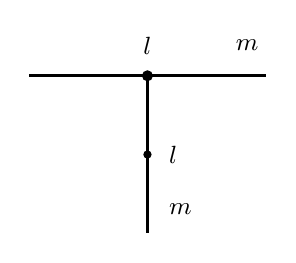
\begin{tikzpicture}[scale=1, font=\small]
  % Problem 5-14: T-shaped cross from two rods of mass m, length l
  % Horizontal rod (top bar)
  \draw[very thick] (-1.5, 2) -- (1.5, 2);

  % Vertical rod
  \draw[very thick] (0, 2) -- (0, 0);

  % Length labels
  \node[above] at (0, 2.15) {$l$};
  \node[right] at (0.15, 1) {$l$};

  % Mass labels
  \node[above right] at (1.0, 2.2) {$m$};
  \node[below right] at (0.15, 0.5) {$m$};

  % Center of horizontal rod
  \fill (0, 2) circle (2pt);

  % Center of vertical rod
  \fill (0, 1) circle (1.5pt);
  \node[right] at (0.15, 1) {};
\end{tikzpicture}
